% !BIB TS-program = biber
% !BIB program = biber
\documentclass[10pt, handout]{beamer}
%\documentclass[10pt]{beamer}

% Packages %
\usepackage[eng]{felipito}
%\usepackage{lmodern}
\usepackage[backend=biber,style=numeric-comp,sorting=none]{biblatex}
%\addbibresource{references.bib}
%\usepackage{coloremoji}

% Theme, color and font
\usetheme{Madrid}	
\usefonttheme{professionalfonts}
\beamertemplatenavigationsymbolsempty

% Epigraph
\setlength{\epigraphwidth}{0.89\textwidth}
\renewcommand{\textflush}{flushepinormal}
\renewcommand {\epigraphflush} {center}
\renewcommand {\sourceflush} {flushleft}

% Title and date
\title[]{Aggregate problems require aggregate solutions?}
\subtitle{When heterogeneity is expendable}
\author{Felipe Del Canto}
\institute[]{Pontificia Universidad Católica de Chile}
\date{\today}

% Graphics path
\graphicspath{{../_Paper/Graphics/}}

% Documento %
\begin{document}

% Portada %
\frame[noframenumbering, plain]{\titlepage}

%: Outline
\begin{frame}[noframenumbering, plain]{Index}
	\tableofcontents
\end{frame}

%%%	Introduction		%%%
\section{Introduction}

%:	Outline
\begin{frame}[t]{Aggregation is an approximation}
	\begin{center}
		\epigraph{\scriptsize (...) all models are approximations. Essentially, all models are wrong, but some are useful. However, %
the approximate nature of the model must always be borne in mind.}{\scriptsize\textit{Empirical Model-Building and Response Surfaces (1987)} \\ \textsc{George Box and Norman Draper}}
	\end{center} 

\pause \vfill
	\begin{itemize}
		\item Aggregate models are, in particular, approximations. \pause \vfill
		\item The conditions to have exact aggregation are strict. \pause \vfill
		\item But the important measure of these models are their predictions. \pause \vfill
		\item Three questions: \vspace{.5ex}
			\begin{itemize}
				\item Is it possible to calibrate aggregate models to obtain better predictions? \vspace{1ex}
				\item How large can be the approximation error when aggregating? \vspace{1ex}
				\item How can we compare aggregate and disaggregate models?
			\end{itemize}
			\vfill
	\end{itemize}
\end{frame}

\begin{frame}{Aggregation ``$=$'' heterogeneity approximation}
	\vfill
	\begin{itemize} 
		\item Typically two types of aggregation are studied:\vspace{.5ex}
			\begin{itemize}
				\item Across consumers (representative agent models). \vspace{1ex}
				\item Across goods (i.e., two good models). 
			\end{itemize} \vfill \pause

		\item But aggregation is just approximating heterogeneity in preferences, income, geography, etc. \vfill \pause
			
		\item Aggregation ``$=$'' approximating distributions of heterogeneous variables:\vspace{.5ex}
			\begin{itemize}
				\item Distribution $F$ is approximated by a Dirac distribution $\delta_{x}$ at the point $x$. \vspace{1ex}
				\item $x$ is the choice of parameters of the aggregate model. 
			\end{itemize} \vfill

	\end{itemize}

\end{frame}

%%%	Aggregation across consumers		%%%
\section{Aggregation across consumers}

%:	Outline
\begin{frame}[noframenumbering, plain]
	\tableofcontents[currentsection]
\end{frame}

\begin{frame}{The economy}
	\vfill
	\begin{itemize}
		\item Two periods ($t \in \{0,1\}$) and two goods ($x_{1t}, x_{2t}$) with prices $(p_{1t},p_{2t}) \in \R^{2}_{++}$. \vfill
		
		\item Agents identified with pairs income-preferences $(y_{t},\alpha_{t})$, with utility function\vspace{1ex}
				$$u_{\alpha_{t}}(x_{1t}, x_{2t}) = x_{1t}^{\alpha_{t}}x_{2t}^{1-\alpha_{t}}.$$\vfill
		
		\item $(y_{t},\alpha_{t}) \sim F_{t}$ (with marginals $F_{x}$, $x = y_{t},\alpha_{t}$) and $\supp F \subset (0,\infty) \times (0,1)$.\vfill
		
		\item Demand for good 1 is $x_{1}(p_{1t}, y_{t} ,\alpha_{t}) = \alpha_{t} y_{t} p_{1t}^{-1}$ and aggregate demand is\vspace{1ex}
				$$X_{1t}(p_{1t}, F_{t}) 
					= \frac{1}{p_{1t}} \int_{S} y_{t}\alpha_{t} \, dF(y_{t},\alpha_{t}) 
					= \frac{1}{p_{1t}}\Big(\mathbb{E}[y_{t}]\mathbb{E}[\alpha_{t}] + \mathrm{Cov}(y_{t},\alpha_{t})\Big).$$\vfill
	\end{itemize}
\end{frame}

\begin{frame}{The researcher's problem and approximation errors}
	\vfill
	\begin{itemize}
		\item Objective: Estimate demand $X_{11}$ using $X_{10}$ and $F_{y_{0}}$.\vfill
		
		\item $F_{\alpha}$ is unknown $\Rightarrow$ use a representative agent (RA) model.\vspace{1ex}
			\begin{itemize}
				\item That is, choose $\overline{\alpha}$ and approximate $F_{\alpha}$ with $\delta_{\overline{\alpha}}$.\footnote[frame]{$\delta_{\overline{\alpha}}$ is the Dirac distribution centered at $\overline{\alpha}$.}
			\end{itemize} \vfill
			
		\item Best estimation for $X_{1t}$ is\vspace{1ex}
				$$\widehat{X}_{1t}(p_{1t}, F_{y_{t}}, \overline{\alpha}) = \overline{\alpha}\, \frac{E[y_{t}]}{p_{1t}}.$$
			\vfill
				
		\item Monetized error at time $t$ is\vspace{1ex}
				$$D_{t}(\overline{\alpha}) 
		 			:=	p_{1t}\Big| X_{1t} - \widehat{X}_{1t}\Big|
					=	\mathbb{E}[y_{t}]\left|\, \mathbb{E}[\alpha_{t}] + \frac{\mathrm{Cov}(y_{t},\alpha_{t})}{\mathbb{E}[y_{t}]} - \overline{\alpha}\,\right|.$$
	\end{itemize} \vfill

\end{frame}

\begin{frame}[label=RA-Example]{Optimal $\overline{\alpha}$ and goodness-of-fit: An example}
	\vfill
	\begin{itemize}
		\item Suppose $\alpha_{0} = \alpha_{1} = \alpha \sim U(0,1)$, and $y_{t} \sim \log\text{-Normal}(10, \sigma_{t})$.\vspace{1ex}
			\begin{itemize}
				\item Joint support is such that for higher $\alpha$, the agent has higher income. \vspace{1ex}
				\item \hyperlink{SupportRA}{\beamerbutton{Joint support}}
			\end{itemize}\vfill
		
		\item From $t = 0$ to $t = 1$, a redistribution of income: $\sigma_{1} \geq \sigma_{0} = 0.25$.\vspace{1ex}
			\begin{itemize}
				\item Median is maintained $\Rightarrow$ Transfer from poor half to rich half. \vspace{1ex}
				\item \hyperlink{DensityRA}{\beamerbutton{Income densities}} 
			\end{itemize} \vfill
			
		\item $\overline{\alpha}$ is chosen at $t = 0$ $\Rightarrow$ $D_{1}(\overline{\alpha})$ is the associated error.\vspace{1ex}
			\begin{itemize}
				\item \hyperlink{alphaBar-RA}{\beamerbutton{Optimal $\overline{\alpha}$}} \vspace{1ex}
				\item \hyperlink{Dt-RA}{\beamerbutton{Approximation error}} 
			\end{itemize} \vfill

	\end{itemize}

\end{frame}



%%%	Aggregation in dynamical models		%%%
\section{Aggregation in dynamic models}

%:	Outline
\begin{frame}[noframenumbering, plain]
	\tableofcontents[currentsection]
\end{frame}

\begin{frame}[label=Carroll-Model]{The model}
	\vfill
	\begin{itemize}
		\item Consumers are pairs $(\beta, \rho)$.\vspace{1ex}
			\begin{itemize}
				\item $\beta$: impatience/discount factor. \vspace{1ex}
				\item $\rho$: relative risk aversion coefficient. 
			\end{itemize} \vfill
		
		 \item They maximize CRRA intertemporal utility subject to accumulation and budget constraints. \hyperlink{Carroll-Program}{\beamerbutton{Optimization problem}} \vfill
			
		\item Interest: estimate $MPC$. Two problems: \vspace{1ex}
			\begin{itemize}
				\item Policy function expression is unknown. \vspace{1ex}
				\item Policy function is highly kinked. \hyperlink{Carroll-Consumption}{\beamerbutton{Policy function}}
			\end{itemize} \vfill
		
		\item Using a RA can be harmful to the estimation. \vspace{1ex}
			\begin{itemize}
				\item Here, $RA$ $\Leftrightarrow$ Choose $\left(\overline{\beta}, \overline{\rho}\right)$ to describe all agents.
			\end{itemize} \vfill

	\end{itemize}
\end{frame}

\begin{frame}[label=Carroll-Example]{An example}
	\vfill
	\begin{itemize}
		\item The economy has 200 agents $(\beta,\rho,y)$ drawn from independent distributions.\vspace{1ex}
			\begin{itemize}
				\item \hyperlink{Carroll-Construction}{\beamerbutton{Economy construction}}.\vspace{1ex}
				\item \hyperlink{Carroll-JointBetaRho}{\beamerbutton{$(\beta, \rho)$ distribution}}, \hyperlink{Carroll-JointAll}{\beamerbutton{$(\beta, \rho, y)$ distribution}}.
			\end{itemize} \vfill

		\item ``Real'' $MPC \approx 0.176$. \vfill
		
		\item RA can produce same $MPC$: \hyperlink{Carroll-MPCgrid}{\beamerbutton{RA $MPC$}}. \vfill
		
		\item For a given tolerance $\epsilon$, several parameters give $error \leq \epsilon$.\vspace{1ex}
			\begin{itemize}
				\item \hyperlink{Carroll-ZeroDiff}{\beamerbutton{``Zero'' difference curves}}.
				\item Difference is more sensitive to $\overline{\beta}$ (smaller range) than $\overline{\rho}$.
			\end{itemize}
 
	\end{itemize} \vfill

\end{frame}


%%%	Representative agent and category goods		%%%
\section{Representative agent and category goods}

%:	Outline
\begin{frame}[noframenumbering, plain]
	\tableofcontents[currentsection]
\end{frame}

\begin{frame}[label=Category-Model]{Description}
	\vfill
	\begin{itemize}
		\item Two periods ($t \in \{0,1\}$) and $n+1$ goods ($\mathbf{x}_{t}, z_{t}$) with prices $(\mathbf{p}_{t},q_{t}) \in \R^{n+1}_{++}$. \vfill
		
		\item Agents identified with pairs income-preferences $(y_{t},\alpha)$, with utility function\vspace{1ex}
	$$u_{\alpha}(\mathbf{x},z) := u_{(y_{t},\alpha)}(\mathbf{x}_{t},z_{t}) = \left(\sum_{j=1}^{n} x_{jt}^{\alpha_{t}}\right)z_{t}^{1-\alpha}.$$		
		\item $(y_{t},\alpha) \sim F_{t}$ (with marginals $F_{x}$, $x = y_{t},\alpha$) and $\supp F_{t} \subset (0,\infty) \times (0,1)$.\vfill
		
		\item Using $X_{t} := g_{\alpha}(\mathbf{x}_{t}) = \|\mathbf{x}_{t}\|_{\alpha}$, $\epsilon = (1-\alpha)^{-1}$ and $P_{\alpha}(\mathbf{p}_{t}) = \|\mathbf{p}_{t}\|_{1-\epsilon}$, demand for category $X_{t}$ is\vspace{1ex}
				$$X_{t}(\mathbf{p}_{t}, y_{t}, \alpha) = yT_{t}(\alpha, \mathbf{p}_{t}) = y\, \frac{\alpha}{P_{\alpha}(\mathbf{p}_{t})}.\footnote[frame]{\hyperlink{Vector-Norms}{\;\beamerbutton{Vector norms}}}$$\vfill
	\end{itemize}

\end{frame}

\begin{frame}[label=Category-Error]{A complex estimation error}
	\vfill
	\begin{itemize}
		\item Objective: Predict $X_{1}$ using RA model. Using $\overline{\alpha}$ the best estimation is
				$$\widehat{X}_{t}(\mathbf{p}_{t}, F_{y_{t}}, \overline{\alpha}) = \mathbb{E}[y_{t}]T_{t} := \mathbb{E}[y_{t}]\, T_{t}(\alpha, \mathbf{p}_{t}).$$
			
		\item Estimation error is
				$$D_{t}\left(\overline{T}_{t}\right)
					:=	\mathbb{E}[y_{t}]\Big\{\tilde{M}_{t} - \overline{T}_{t}\Big\}
					=	\mathbb{E}[y_{t}]\left\{ \frac{\mathrm{Cov}\left(y_{t}, T_{t} \right)}{\mathbb{E}[y_{t}]} + \mathbb{E}\left[T_{t}\right] - \overline{T}_{t} \right\}.
				$$
				\vfill
		
		\item The important distribution is that of $(y_{t}, T_{t})$ $\Rightarrow$ Now heterogeneity in $\mathbf{p}_{t}$ is important. \vfill

		\item If relative prices are constant between periods, a correction can be made.\vspace{1ex}
			\begin{itemize}
				\item If $\mathbf{p}_{1} = \lambda \mathbf{p}_{0}$.\vspace{1ex}
				\item Set $\overline{T}_{0} = \tilde{M}_{0}$, then $\overline{T}_{1} = \lambda^{-1}\overline{T}_{0}$.\vspace{1ex}
				\item \hyperlink{Category-OptimalityCondition}{\beamerbutton{Optimality Condition}}
			\end{itemize}

	\end{itemize} \vfill

\end{frame}

\begin{frame}[label=Category-Example]{Numerical example}
	\vfill
	\begin{itemize}
		\item Suppose $\alpha_{0} = \alpha_{1} = \alpha \sim U(0.15,0.85)$, and $y_{t} \sim \log\text{-Normal}(\log 5.5, \sigma_{t})$.\vspace{1ex}
			\begin{itemize}
				\item For higher $\alpha$, agent has higher income. \hyperlink{Category-Support}{\beamerbutton{Joint support}} \vspace{1ex}
				\item From $t = 0$ to $t = 1$ redistribution: $\sigma_{1} \geq \sigma_{0} = 0.25$
			\end{itemize}\vfill
		
		\item From $t = 0$ to $t = 1$, $\mathbf{p}_{1} = \lambda \mathbf{p}_{0}$. \vspace{1ex}
			\begin{itemize}
				\item Compare $\lambda_{1} = 0.5$ and $\lambda_{2} = 1.5$.\vspace{1ex}
				\item Set $\mathbf{p}_{0} = (1,10)$.\vspace{1ex}
				\item \hyperlink{Category-TbyP}{\beamerbutton{$T_{t}$ by price}}
			\end{itemize} \vfill
		
		\item $\overline{\alpha}$ is chosen at $t = 0$ $\Rightarrow$ $\overline{T}_{1} = \lambda_{i}^{-1} \overline{T}_{0}$ $\Rightarrow$ $D_{1}(\overline{T}_{1})$ is the error.\vspace{1ex}
			\begin{itemize}
				\item $\mathrm{Cov}(y_{t}, T_{t})$ is small, close to $10^{-15}$.\vspace{1ex}
				\item Low variance of $\overline{\alpha}$. \hyperlink{Category-alphaBar}{\beamerbutton{Optimal $\overline{\alpha}$}} \vspace{1ex}
				\item $D_{1}(\overline{T}_{1}) \approx 0$. \hyperlink{Category-Dt}{\beamerbutton{Approximation error}}
			\end{itemize} \vfill

	\end{itemize}

\end{frame}


%%%	Final remarks		%%%
\section{Final remarks}


%:	Outline
\begin{frame}[noframenumbering, plain]
	\tableofcontents[currentsection]
\end{frame}

\begin{frame}{Final remarks}
	\vfill
	\begin{itemize}
		\item Aggregation is heterogeneity approximation.\vspace{1ex}
			\begin{itemize}
				\item Hence, we have a spectrum.\vspace{1ex}
				\item Between a distribution $F$ and $\delta_{x}$ there are infinite choices.
			\end{itemize} \vfill

		\item Two factors to determine approximate distribution $\widehat{F}$:\vspace{1ex}
			\begin{itemize}
				\item Variable to estimate.\vspace{1ex}
				\item Accuracy desired.
			\end{itemize} \vfill

		\item For a given precision, what is needed is a finite number of moments of $F$.\vspace{1ex}
			\begin{itemize}
				\item For example, the moments given by a Taylor approximation.\vspace{1ex}
				\item Hence, all is needed is a model with $\widehat{F}$ with those moments.\vspace{1ex}
				\item Or a simpler $\widehat{F}$ that has a specific moment (e.g., RA models).
			\end{itemize}
	\end{itemize} \vfill

\end{frame}


%:Back cover
\begin{frame}[plain,noframenumbering]
  \titlepage
 \end{frame}

%:Annex
\section*{Annex}

\begin{frame}[label=SupportRA,plain,noframenumbering]{\secname: Joint Distributions (Representative agent)\,\hyperlink{RA-Example}{\beamerreturnbutton} }
	\begin{figure}[H] 
		\caption{Support of $F_{0}$ and $F_{1}$}
		\label{fig:JointDistributions}
		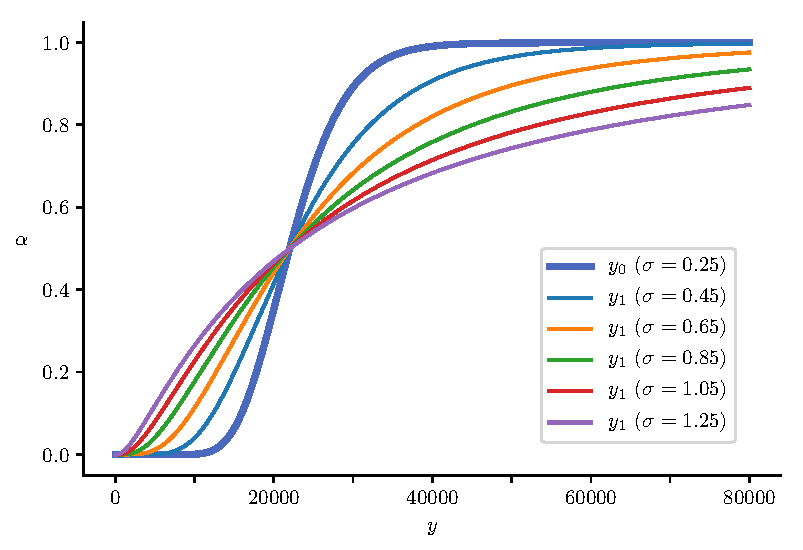
\includegraphics[width = 0.6\textwidth]{RAjointDistribs}
		\floatfoot{\begin{minipage}{0.6\textwidth}
			The thick line represents the joint distribution at $t = 0$. The thin lines are five different examples of joint distributions at $t = 1$, varying in the value of $\sigma_{1}$.
		\end{minipage}}
	\end{figure}
\end{frame}

\begin{frame}[label=DensityRA,plain,noframenumbering]{\secname: Income density (Representative agent)\,\hyperlink{RA-Example}{\beamerreturnbutton} }
	\begin{figure}[H] 
		\caption{Densities of $y_{0}$ and $y_{1}$ for different values of $\sigma_{1}$.}
		\label{fig:LogNormalSigma1}
		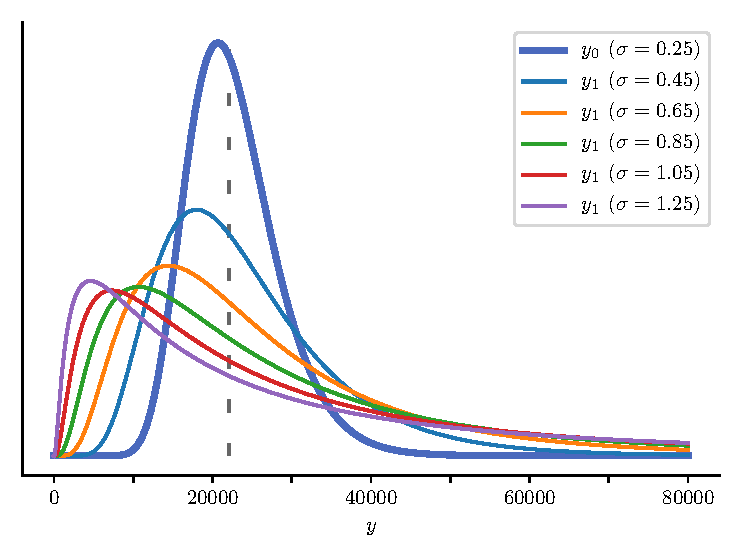
\includegraphics[width = 0.6\textwidth]{RAwageDistribs} \vspace{-1.4ex}
		\floatfoot{\begin{minipage}{0.6\textwidth}
			All distributions have $\mu = 10$ and $\sigma$ according to the legend. The thick line represents the income distribution at $t = 0$. The thin lines are five different examples of distributions at $t = 1$. The dashed gray line corresponds to the common median at, approximately, 22\,026.
		\end{minipage}}
	\end{figure}
\end{frame}

\begin{frame}[label=alphaBar-RA,plain,noframenumbering]{\secname: Optimal $\overline{\alpha}$ (Representative agent)\,\hyperlink{RA-Example}{\beamerreturnbutton} }
	\begin{figure}[H] 
		\caption{Optimal $\overline{\alpha}$ at $t = 1$ as a function of $\sigma$.}
		\label{fig:RAoptimalAlphas}
		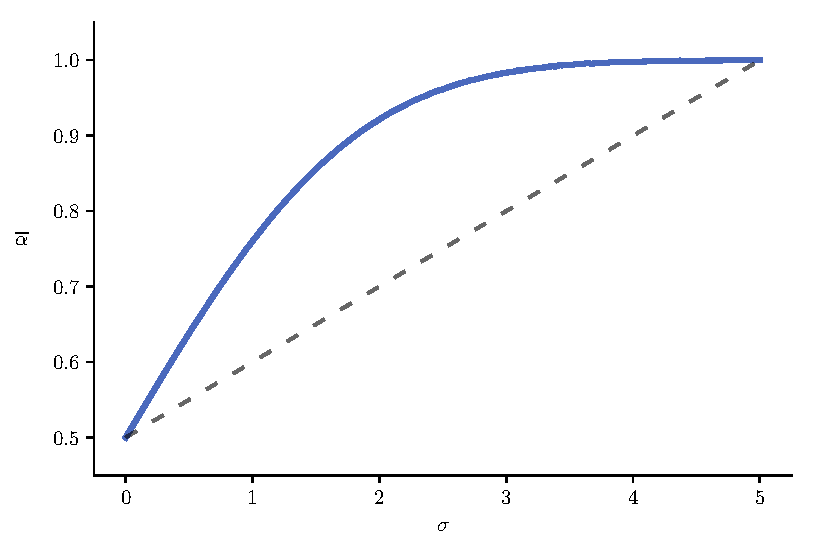
\includegraphics[width = 0.6\textwidth]{RAoptimalAlphas}
		\floatfoot{\begin{minipage}{0.6\textwidth}
			The blue line shows the optimal $\overline{\alpha}$ as a function of $\sigma$, with $\alpha \sim U(0,1)$ and $y \sim \log\text{-Normal}(\mu, \sigma)$, with $\mu = 10$. The dashed gray line joins the two extremes of the curve.
		\end{minipage}}
	\end{figure}
\end{frame}

\begin{frame}[label=Dt-RA,plain,noframenumbering]{\secname: Approximation error (Representative agent)\,\hyperlink{RA-Example}{\beamerreturnbutton} }
	\begin{figure}[H] 
		\caption{Estimation error $D(\overline{\alpha})$ as a function of $\sigma_{1}$.}
		\label{fig:RADiffPlot}
		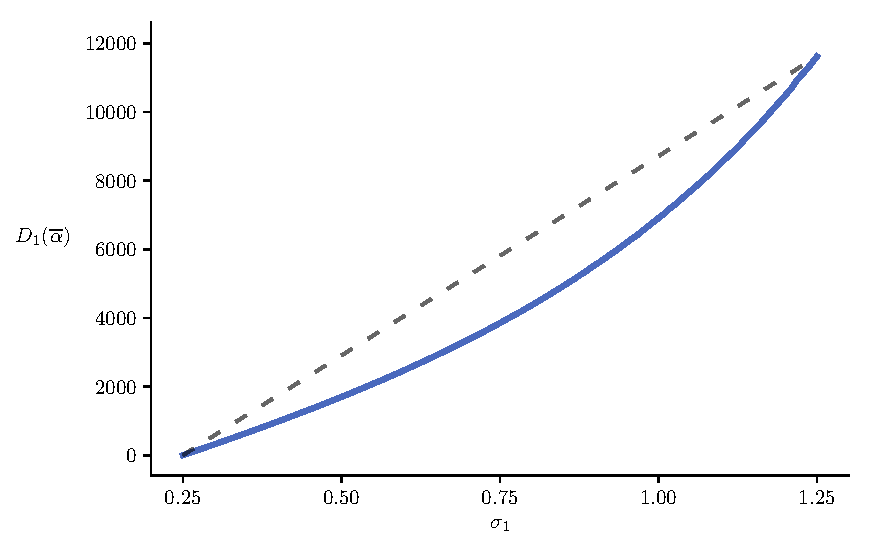
\includegraphics[width = 0.6\textwidth]{RAdiffPlot}
		\floatfoot{\begin{minipage}{0.6\textwidth}
			The blue line shows $D(\overline{\alpha})$ as a function of $\sigma_{1}$. The dashed gray line corresponds joins the two extremes of the curve.
		\end{minipage}}
	\end{figure}
\end{frame}

\begin{frame}[label=Carroll-Program, plain, noframenumbering]{\secname: Agent Program (Dynamic models)\,\hyperlink{Carroll-Model}{\beamerreturnbutton}}
	\vfill
	\begin{itemize}
		\item The agent solves \vspace{2ex}
				$$\probop{\max_{\{c_{t}\}_{t}}}{\sum_{t=1}^{\infty} \beta^{t}\frac{c_{t}^{1-\rho}}{1-\rho}}
					{&	k_{t+1} = (1-\delta)(y_{t} - c_{t+1})	\\
					&	y_{t} = k_{t} + \theta_{t}k_{t}^{\alpha}},$$
			where \vspace{1ex}
			\begin{itemize}
				\item $c_{t}$ is the consumption at time $t$, \vspace{1ex}
				\item $k_{t}$ is the capital at time $t$, \vspace{1ex}
				\item $y_{t}$ is income at tiem $t$, \vspace{1ex}
				\item $\theta_{t}$ is a permanent production growth factor. 
			\end{itemize} \vfill
			
		\item All lower-cap variables are normalized by permanent labor income, $wL$.
	\end{itemize}

\end{frame}

\begin{frame}[label=Carroll-Consumption, plain, noframenumbering]{\secname: Policy Function (Dynamic models)\,\hyperlink{Carroll-Model}{\beamerreturnbutton}}
	\begin{figure}[H]
		\caption{Consumption function}
		\label{fig:concaveC}
		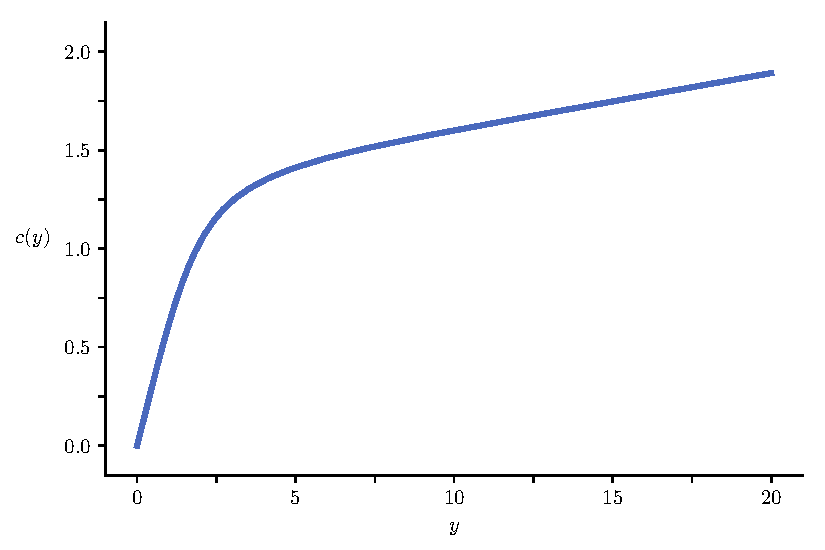
\includegraphics[width=0.8\textwidth]{CarrollCons}
		%\floatfoot{Note}
	\end{figure}
\end{frame}

\begin{frame}[label=Carroll-Construction, plain, noframenumbering]{\secname: Economy Construction (Dynamic models)\,\hyperlink{Carroll-Example}{\beamerreturnbutton}}
	\vfill
	\begin{itemize}
		\item Each agent is a triple $(\beta,\rho,y)$. \vfill
		
		\item Take 200 draws independently from the following distributions\vspace{1ex}
				\begin{itemize}
					\item $\beta$: triangular distribution with lower limit $0.9$ and with upper limit and mean equal to $0.99$. \vspace{2ex}
					\item $\rho$: triangular distribution with lower limit $1$, upper limit $5$ and mean $3$. \vspace{2ex}
					\item $y$: uniform distribution over the interval $[0,10]$. 
				\end{itemize} \vfill
							
		\item The previous construction ensure all variables are independent.
	\end{itemize}

\end{frame}

\begin{frame}[label=Carroll-JointBetaRho, plain, noframenumbering]{\secname: $(\beta, \rho)$ distribution (Dynamic models)\,\hyperlink{Carroll-Example}{\beamerreturnbutton}}
	\begin{figure}[H]
		\caption{Distribution of $\beta$ and $\rho$ in the economy.}
		\label{fig:distribBetaRho}
		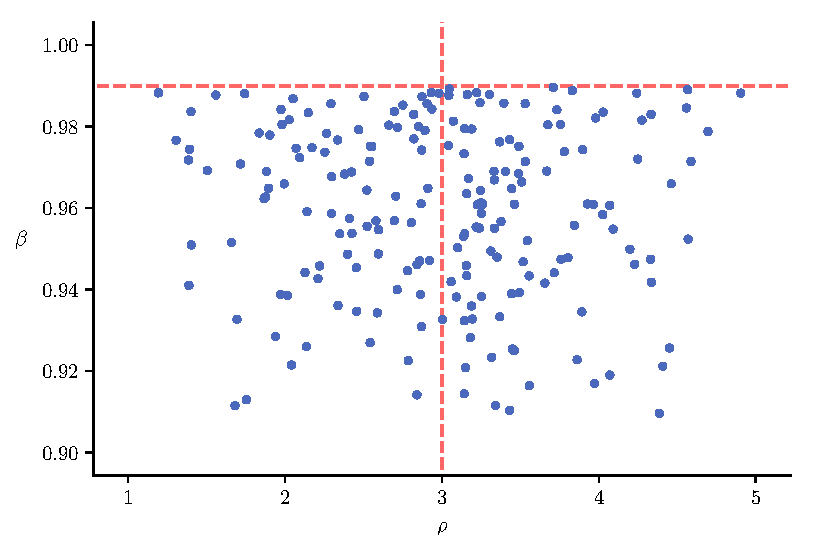
\includegraphics[width=0.6\textwidth]{CarrollDistrib}
		\floatfoot{\begin{minipage}{0.6\textwidth}
			The figure shows the marginal distribution $F_{\beta,\rho}$. Each dot represents an agent in the economy. The dashed lines correspond to $\rho = 3$ and $\beta = 0.99$, the means of the triangular distributions.
		\end{minipage}}
	\end{figure}
\end{frame}

\begin{frame}[label=Carroll-JointAll, plain, noframenumbering]{\secname: $(\beta, \rho, y)$ distribution (Dynamic models)\,\hyperlink{Carroll-Example}{\beamerreturnbutton}}
	\begin{figure}[H]
		\caption{Joint distribution of $\beta$, $\rho$ and $y$ in the economy.}
		\label{fig:JointDistrib}
		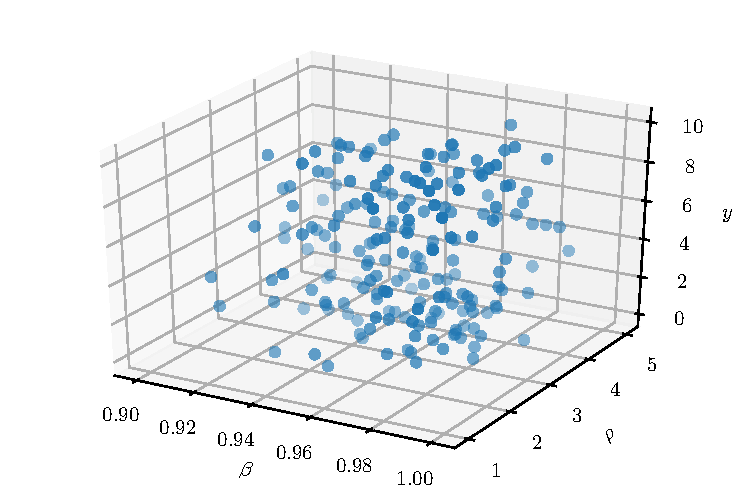
\includegraphics[width=0.6\textwidth]{CarrollDistrib3d}
		\floatfoot{\begin{minipage}{0.6\textwidth}
			The figure shows the distribution $F_{\beta,\rho,y}$. Each dot represents an agent in the economy.
		\end{minipage}}
	\end{figure}
\end{frame}

\begin{frame}[label=Carroll-MPCgrid, plain, noframenumbering]{\secname: RA $MPC$ (Dynamic models)\,\hyperlink{Carroll-Example}{\beamerreturnbutton}}
	\begin{figure}[H]
		\caption{Computed MPC for each pair $(\overline{\beta}, \overline{\rho})$.}
		\label{fig:MPCPlane}
		\includegraphics[width=0.6\textwidth]{CarrollMPC}
		\floatfoot{\begin{minipage}{0.6\textwidth}
			The figure shows the computed MPC for each pair $\left(\overline{\beta}, \overline{\rho}\right)$ in a 10\,000 point grid constructed in $[0.9, 1] \times [1,5]$. The red plane is set at the real value of the MPC for this economy, approximately at 0.176. 
		\end{minipage}}
	\end{figure}
\end{frame}

\begin{frame}[label=Carroll-ZeroDiff, plain, noframenumbering]{\secname: ``Zero'' difference curves (Dynamic models)\,\hyperlink{Carroll-Example}{\beamerreturnbutton}}
	\begin{figure}[H]
		\caption{``Zero'' difference curves}
		\label{fig:ZeroCurve}
		
		\subfloat[tolerance = $10^{-4}$]{\includegraphics[width=0.45\textwidth]{CarrollMPCCurve_-4}}
		\subfloat[tolerance = $10^{-5}$]{\includegraphics[width=0.45\textwidth]{CarrollMPCCurve_-5}} \vspace{-2ex}

		\floatfoot{\begin{minipage}{0.9\textwidth}
			The figure shows pairs $(\overline{\beta}, \overline{\rho})$ for which $|D(\overline{\beta}, \overline{\rho})|$ is less or equal than a certain tolerance. In Panel (a) the tolerance is $10^{-4}$ and in Panel (b) the tolerance is $10^{-5}$.
		\end{minipage}}
	\end{figure}
\end{frame}

\begin{frame}[label=Category-OptimalityCondition,plain,noframenumbering]{\secname: Optimality of correction (Category goods)\,\hyperlink{Category-Error}{\beamerreturnbutton}}
	\vfill
	\begin{itemize}
		\item If $\mathbf{p}_{1} = \lambda \mathbf{p}_{0}$, then
				$$T_{1} = \lambda^{-1}T_{0},$$
			and thus
				$$\lambda^{-1}\tilde{M}_{0} = \mathbb{E}[T_{1}] + \frac{\mathrm{Cov}\left(y_{0}, T_{1} \right)}{\mathbb{E}[y_{0}]}.$$ \vfill
	
		\item The correction $\overline{T}_{1} = \lambda^{-1}\overline{T}_{0}$ reduces the error if
				\begin{small}$$\begin{aligned}
					\left|\tilde{M}_{1} - \lambda^{-1}\tilde{M}_{0} \right|
						&\leq \left|\tilde{M}_{1} - \tilde{M}_{0} \right|	\\
					\left| \frac{\mathrm{Cov}\left(y_{1}, T_{1} \right)}{\mathbb{E}[y_{1}]} - \frac{\mathrm{Cov}\left(y_{0}, T_{1} \right)}{\mathbb{E}[y_{0}]} \right|
						&\leq \left| \mathbb{E}\left[T_{1} \right] - \mathbb{E}\left[T_{0} \right] + \frac{\mathrm{Cov}\left(y_{1}, T_{1} \right)}{\mathbb{E}[y_{1}]} - \frac{\mathrm{Cov}\left(y_{0}, T_{0} \right)}{\mathbb{E}[y_{0}]} \right|	\\
					\left| \frac{\mathrm{Cov}\left(y_{1}, T_{1} \right)}{\mathbb{E}[y_{1}]} - \frac{\mathrm{Cov}\left(y_{0}, T_{1} \right)}{\mathbb{E}[y_{0}]} \right|
						&\leq \left| (1-\lambda)\mathbb{E}\left[T_{1} \right] + \frac{\mathrm{Cov}\left(y_{1}, T_{1} \right)}{\mathbb{E}[y_{1}]} - \frac{\mathrm{Cov}\left(y_{0}, T_{0} \right)}{\mathbb{E}[y_{0}]} \right|.
				\end{aligned}$$\end{small} \vfill
	\end{itemize}
\end{frame}

\begin{frame}[label=Category-Support,plain,noframenumbering]{\secname: Joint Distributions (Category goods)\,\hyperlink{Category-Example}{\beamerreturnbutton} }
	\begin{figure}[H]
		\caption{Support of joint distributions of $y_{t}$ and $T_{t}$.}
		\label{fig:JointDistribsCategory}		
		\subfloat[$(y_{t},T_{t}), \lambda_{1} = 0.5$]{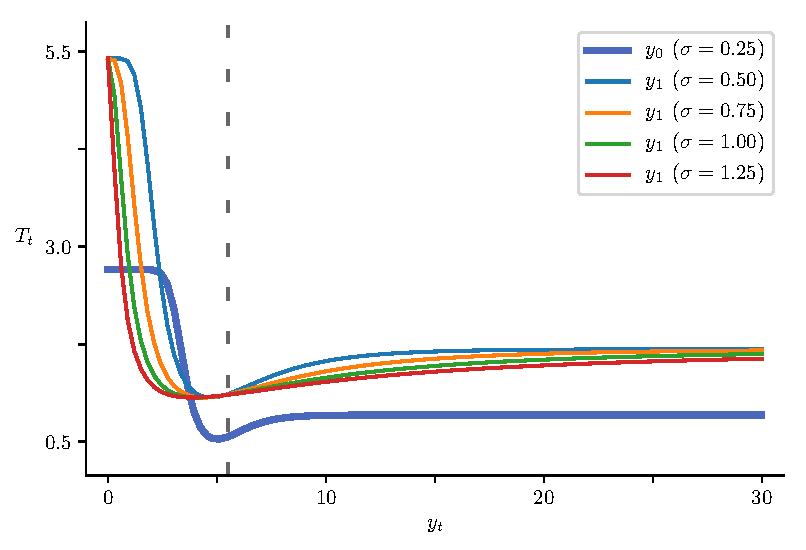
\includegraphics[width = 0.45\textwidth]{JointYT_0}\label{fig:Jointb}}\,
		\subfloat[$(y_{t},T_{t}), \lambda_{2} = 1.5$]{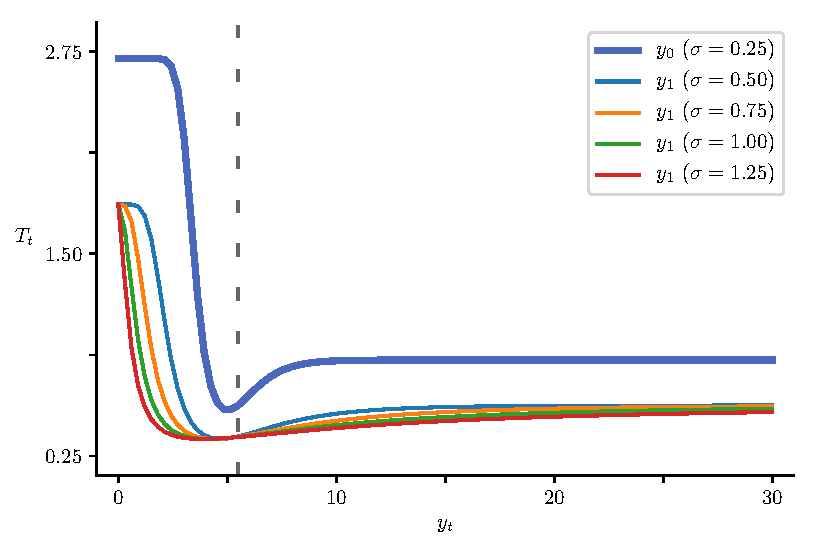
\includegraphics[width = 0.45\textwidth]{JointYT_1}\label{fig:Jointc}}
		\vspace{-2ex}
		\floatfoot{\begin{minipage}{0.9\textwidth} The figure shows the support of the joint distributions of $(y_{t}, \alpha)$, $(y_{t}, T_{t})$ with $\lambda = 0.5$ and $(y_{t}, T_{t})$ with $\lambda = 0.5$ for five different values of $\sigma_{1}$. The dashed gray lines correspond to $y_{t} = 5.5$, the median of the distribution.
		\end{minipage}}
	\end{figure}
\end{frame}

\begin{frame}[label=Category-TbyP,plain,noframenumbering]{\secname: $T_{t}$ by price (Category goods)\,\hyperlink{Category-Example}{\beamerreturnbutton}}
	\begin{figure}[H]
		\caption{$T_{0}$ and $T_{1}$ as a function of $\alpha$.}
		\label{fig:DiffTtLambda}
		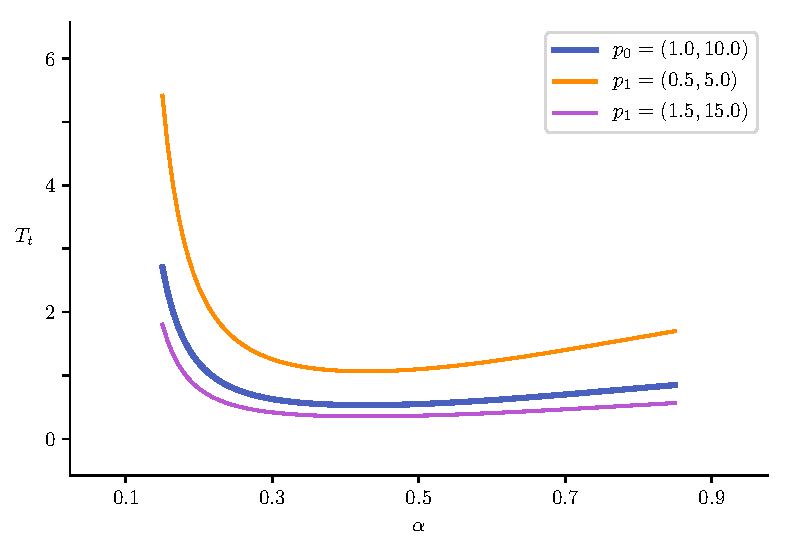
\includegraphics[width = 0.6\textwidth]{TtLambdas}
		\floatfoot{\begin{minipage}{0.6\textwidth} The figure shows $T_{0}$ and $T_{1}$ as a function of $\alpha$. $T_{0}$ is computed using $\mathbf{p}_{0} = (1,10)$ and each $T_{1}$ is computed with $\mathbf{p}_{1} = \lambda_{i}\mathbf{p}_{0}$, where $\lambda_{1} = 0.5$ and $\lambda_{2} = 1.5$.
		\end{minipage}}
	\end{figure}
\end{frame}


\begin{frame}[label=Category-alphaBar,plain,noframenumbering]{\secname: Optimal $\overline{\alpha}$ (Category goods)\,\hyperlink{Category-Example}{\beamerreturnbutton} }
	\begin{figure}[H] 
		\caption{Optimal $\overline{\alpha}$ at $t = 1$ as a function of $\sigma_{1}$.}
		\label{fig:CategoryAlphaPlot}
		\subfloat[$\lambda = 0.5$]{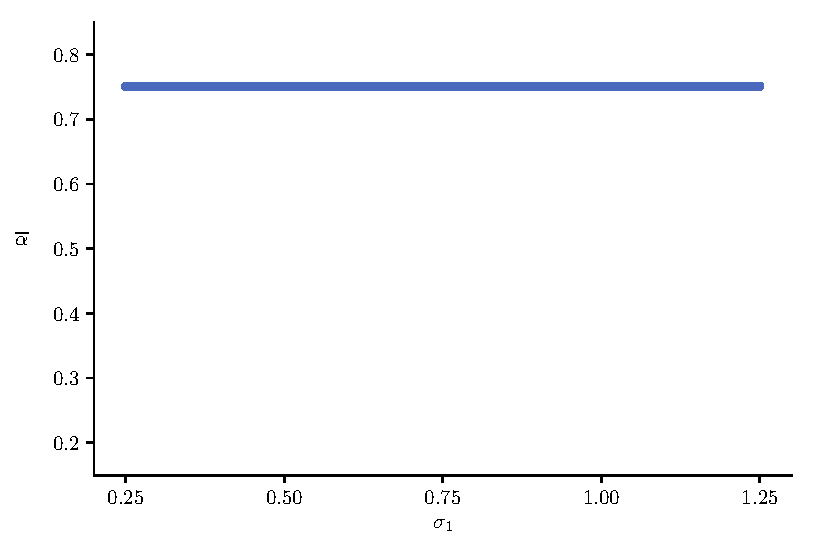
\includegraphics[width = 0.45\textwidth]{CategoryAlphasPlot_0} \label{fig:AlphaCata}}\,
		\subfloat[$\lambda = 1.5$]{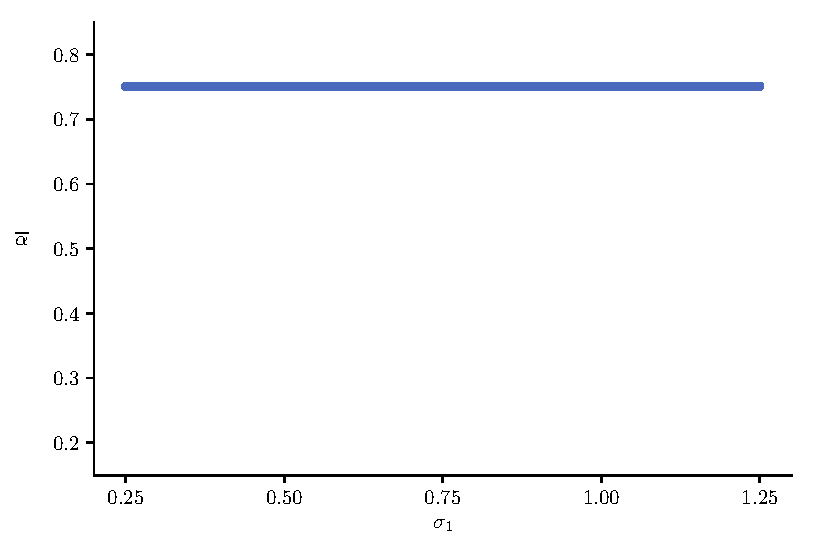
\includegraphics[width = 0.45\textwidth]{CategoryAlphasPlot_1} \label{fig:AlphaCatb}}
		\floatfoot{\begin{minipage}{0.9\textwidth}
			The blue line shows the optimal $\overline{\alpha}$ at $t = 1$ as a function of $\sigma_{1}$. Note that for $\sigma_{1} = 0$, the optimal value of $\overline{\alpha}$ is the same as the one computed at $t = 0$: $0.75$.
		\end{minipage}}
	\end{figure}
\end{frame}

\begin{frame}[label=Category-Dt,plain,noframenumbering]{\secname: Approximation error (Category goods)\,\hyperlink{Category-Example}{\beamerreturnbutton} }
	\begin{figure}[H] 
		\caption{Estimation error $D(\overline{T}_{1})$ as a function of $\sigma_{1}$.}
		\label{fig:CategoryDiff1Plot}
		\subfloat[$\lambda = 0.5$]{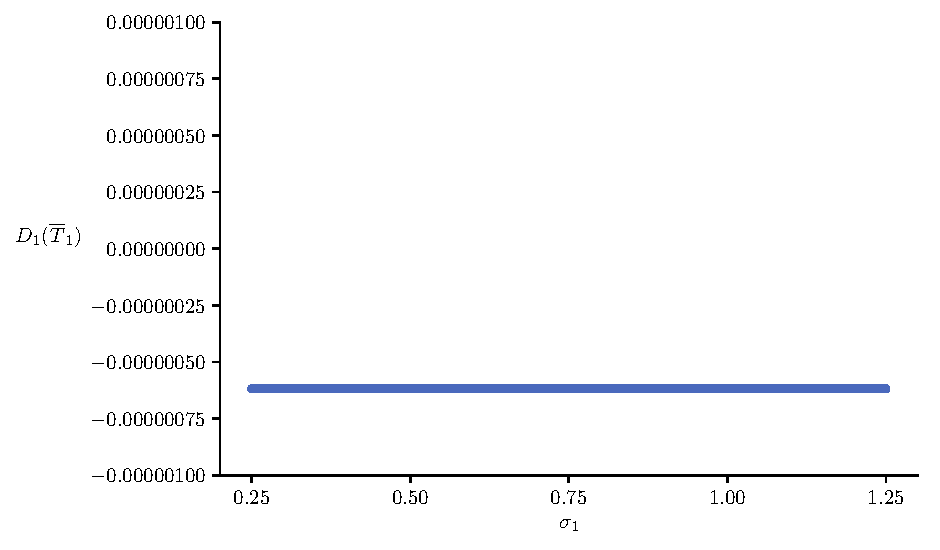
\includegraphics[width = 0.45\textwidth]{Categorydiff1Plot_0} \label{fig:Diffa}}\,
		\subfloat[$\lambda = 1.5$]{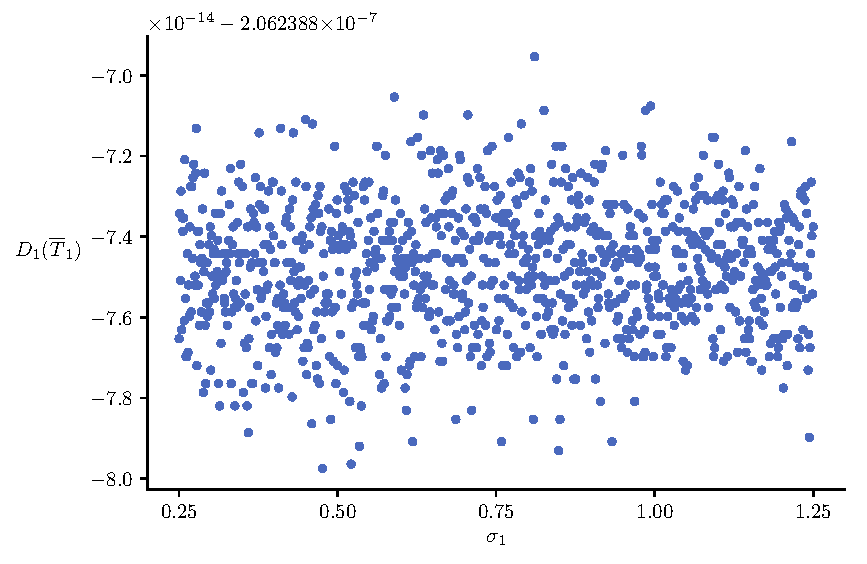
\includegraphics[width = 0.45\textwidth]{Categorydiff1Plot_1} \label{fig:Diffb}}
		\floatfoot{\begin{minipage}{0.9\textwidth}
			The blue dots show $D(\overline{T}_{1})$ as a function of $\sigma_{1}$.
		\end{minipage}}
	\end{figure}
\end{frame}


\begin{frame}[label=Vector-Norms,plain,noframenumbering]{Vector norms\,\hyperlink{Category-Model}{\beamerreturnbutton}}
	\vfill
	\begin{itemize}
		\item For $\mathbf{x} \in \mathbb{R}^{n}_{++}$, $0 < \alpha < \infty$
				$$\|\mathbf{x}\|_{\alpha} := \left(\sum_{j=1}^{n} x_{j}^{\alpha} \right)^{1/\alpha}.$$
				\vfill
			
		\item For $\alpha = \infty$ is it possible to define
				$$\|\mathbf{x}\|_{\infty} := \max_{j} x_{j},$$
			and $\|\mathbf{x}\|_{\infty} = \lim_{a \to \infty} \|\mathbf{x}\|_{\alpha}$.
				\vfill
		
		\item For $1\leq \alpha \leq \infty$, $\|\mathbf{x}\|_{\alpha}$ is a norm.
	\end{itemize}
	\vfill

\end{frame}


\end{document}

